\Chapter{Resultaten\label{hfdst-resultaten}}

In dit hoofdstuk zal het ASIC ontwerp van de schakeling die in \refhfdst{hfdst-implementatie} beschreven werd van naderbij bestudeerd worden. Daarbij zal gekeken worden naar de oppervlakte van de schakeling, het verbruik en de maximum bereikbare kloksnelheid $f_{\text{max}}$. Er zal onderzocht worden wat het effect van de verschillende voorgestelde optimalisaties is op al deze parameters. Ten slotte zal het ontwerp vergeleken worden met reeds bestaande implementaties.

Het ontwerp werd geprogrammeerd in GEZEL \cite{gezel}. Simulaties en compilatie naar VHDL werden uitgevoerd met GEZEL 2.0. De optimalisaties werden doorgevoerd in de VHDL code, aangezien GEZEL dit niet toelaat. Alle ontwerpen werden gesynthetiseerd met behulp van Synopsys Design Vision. De gebruikte bibliotheek was de \emph{$0.13 \mu m$ low leakage} bibliotheek van Faraday Technology \cite{cell-databook}. Het werd de software verboden flip-flops met test ingangen te gebruiken. De maximale oppervlakte werd ingesteld op nul, wat als netto effect een resultaat met minimum oppervlakte gaf. Verder werd voor het kloksignaal een frequentie van 10kHz gedefini\"eerd.

De grootte van alle resultaten wordt uitgedrukt in gates. Dit laat toe te vergelijken met andere resultaten die in de literatuur terug te vinden zijn.

Voor de resultaten in verband met energieverbruik worden steeds twee waarden gegeven. De eerste waarde, dynamisch verbruik, geeft weer hoeveel vermogen verbruikt wordt door veranderende CMOS in- en uitgangen. De tweede waarde, leakage verbruik, is verbruik dat voorkomt zelfs indien een transistor niet geleidt. De impact hiervan hangt onder meer af van de gebruikte bibliotheek.

Deze beide waarden moeten met een stevige korrel zout genomen worden. Het is voor het synthese programma zeer moeilijk hier een nauwkeurige schatting voor te geven. Zolang twee schakelingen echter met dezelfde software, bibliotheek en parameters werden gesynthetiseerd, zijn relatieve vergelijkingen mogelijk. Stel bijvoorbeeld dat het verbruik van ontwerp A geschat wordt op $200 nW$ en dit van ontwerp B op $100 nW$. Indien er dan voldaan is aan de voorgenoemde voorwaarden, zal het effectief verbruik van B ongeveer de helft zijn van A. Het is dus in het algemeen niet aangeraden vergelijkingen omtrent verbruik te maken met andere bestaande ontwerpen aan de hand van de waarden gegeven in dit hoofdstuk.

% TODO: Blijft leakage constant bij hogere kloksnelheid?

Indien gewenst kan het verbruik voor hogere kloksnelheiden geschat worden. Gegeven de standaard frequentie $f = 10$kHz, de formule voor het dynamisch verbruik van een CMOS schakeling:
\[P_d = V^2 \cdot C \cdot f\]
en het leakage verbruik $P_l$, kan men dus het totale verbruik omrekenen naar dat van een willekeurige kloksnelheid via
\[P' = \frac{P_d \cdot f'}{10 000} + P_l.\]

\section{Basisimplementatie \& register optimalisaties\label{section-resultaten-basisimplementatie}}

Het synthetiseren van de meest eenvoudige implementatie, zonder enige optimalisaties aan de registers en met slechts \'e\'en MALU in de $\mathbb{F}_{2^m}$ kern, geeft de resultaten in \reftbl{tabel-resultaten-basis}.


Allereerst zal onderzocht worden wat de effecten zijn van de optimalisaties voorgesteld in \refsect{sectie-implementatie-optimalisatie}. Bij de implementaties met clock gating werden steeds ook de reset ingangen van zoveel mogelijk registers verwijderd. De synthese resultaten voor de vijf verschillende implementaties worden gegeven in \reftbl{tabel-resultaten-optimalisaties}. De versies met clock gating (CG $n$) implementeren de schakelingen in de volgorde waarin ze voorkomen in \refsect{subsectie-implementatie-optimalisatie-clock-gating}. Ter verduidelijking zijn de oppervlakte en het totale verbruik van deze resultaten ook nog eens uitgezet in \reffig{figuur-resultaten-m1}.

%De synthese software gebruikt in de basis implementatie en die zonder reset ingangen flip flops met een enable ingang. Zo'n flip flops kosten achtentwintig gates, waarbij de reset ingang door twee van die gates gevormd wordt. Intern zijn deze flip flops equivalent aan een flip flop zonder enable ingang die naar zichzelf is terug gekoppeld via een multiplexer. Het enable signaal vervult in dit geval de functie van selectie signaal die anders voor de multiplexer nodig zou zijn. De synthese software zal zelf de sturing van de enable signalen bepalen in dit gevallen. Het is om deze reden dat het toepassen van clock gating in dit geval geen oppervlakte winst oplevert tegenover.

Zoals verwacht resulteert het toepassen van clock gating wel in een zeer grote besparing op het verbruik. Daarbij is het opmerkelijk dat het dynamisch verbruik van CG 3 niet lager is dan dat van de andere twee implementaties met clock gating. Het is mogelijk dat de synthese software bij de berekening van het verbruik niet nauwkeurig genoeg te werk gaat om het effect van de clock gating schakeling op de interne gates van de flip flop juist in te schatten. Door het kloksignaal door de clock gating schakelingen te sturen, wordt het als het ware gebufferd. Aangezien in de schakeling het kritische pad gevormd wordt door onder meer het klokpad, zorgt het toepassen van clock gating er dus voor dat het kritische pad verkort wordt.  Dit is de reden waarom de ontwerpen CG $n$ sneller kunnen werken. Waarom de schakeling zonder resets ook een hogere snelheid behaald kan worden, is niet volledig duidelijk.

\begin{table}[h]
	\caption{Syntheseresultaten voor ontwerpen met \'e\'en MALU}
	\label{tabel-resultaten-optimalisaties}

	\centering
	\begin{tabular}{ll@{$\;\;$}rl@{$\;\;$}rl@{$\;\;$}rl@{$\;\;$}r}
		\toprule
		\multirow{2}{*}{Ontwerp}	& \multicolumn{2}{l}{\multirow{2}{*}{Opp. [gates]}}	& \multicolumn{4}{c}{Verbruik @ 10kHz [$nW$]}	& \multicolumn{2}{l}{\multirow{2}{*}{$f_{\text{max}}$ [MHz]}}\\
		\cmidrule{4-7}
		&	& & \multicolumn{2}{l}{Dynamisch}	& \multicolumn{2}{l}{Leakage}	& &\\
		\midrule
		Basis			& $28\,876$	& 			& 512	&	 		& 117 & 			& 50.10 	& \\
		Geen reset	& $27\,596$	& 96\%	& 395	& 77\%	& 107 & 92\%	& 52.11	& 104\%\\
		CG 1			& $27\,751$	& 96\%	& 94	& 18\%	& 109	& 94\%	& 51.68	& 103\%\\
		CG 2			& $27\,713$	& 96\%	& 59	& 12\%	& 102	& 88\%	& 53.76	& 107\%\\
		CG 3			& $27\,734$	& 96\%	& 96	& 19\%	& 110	& 94\%	& 51.65	& 103\%\\
		\bottomrule		
	\end{tabular}
\end{table}

\begin{figure}[h]
	\centering
		\fbox{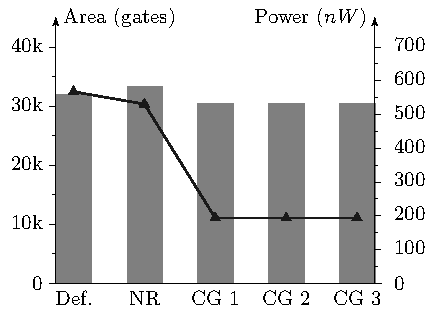
\includegraphics[scale=1]{results-m1}}
		\caption{Syntheseresultaten voor de basis implementatie met en zonder register optimalisaties\label{figuur-resultaten-m1}}
\end{figure}

\section{Meerdere MALU's\label{sectie-resulaten-malus}}

Mits de toevoeging van extra MALU's is het mogelijk de totale rekeningtijd drastisch te verlagen (zie \refsect{subsectie-implementatie-gf2m-versnelling}). Hoewel het gebruik van meerdere MALU's de uiteindelijke schakeling vergroot en dat dus enigszins in gaat tegen de originele doelstelling, wordt hier toch onderzocht in welke mate de interessante parameters hierdoor juist worden be\"invloed. Er kan dan een afweging gemaakt worden tussen het gebruik van een schakeling met \'e\'en MALU op hogere kloksnelheid versus \'e\'en met meerdere MALU's aan een lagere kloksnelheid. De eerste schakeling zal kleiner zijn, maar waarschijnlijk wel meer verbruiken dan de tweede.

De totale berekeningstijd $t = \frac{c}{f}$ kan bepaald worden in functie van het aantal benodigde klokcycli $c$, wat op zijn beurt bepaald wordt door het aantal MALU's $d$:
\[c = 27058 + 2993 \cdot \left\lceil \frac{163}{d} \right\rceil,\]
waarbij 2993 het aantal vermenigvuldigingen is dat dient uitgevoerd te worden en de tweede term in de vermenigvuldiging het aantal klokcycli is die een vermenigvuldiging kost. In \reftbl{tabel-resultaten-multi-cycles} wordt voor enkele waarden getoond hoeveel klokcycli nodig zijn om een berekening te voltooien. In \reffig{figuur-resultaten-multi-cycles} wordt hetzelfde weergegeven, maar dan voor elke $d$ van 1 t.e.m.\ 163. Het is duidelijk dat de tijdsbesparing waar extra MALU's voor zorgen vrij snel teniet wordt gedaan door het aantal cycli dat niet door $d$ be\"invloed wordt.

\begin{table}[h]
	\caption{Aantal klokcycli $c$ nodig voor \'e\'en pairing i.f.v.\ aantal MALU's $d$}
	\label{tabel-resultaten-multi-cycles}

	\begin{narrow}{-1cm}{-1cm}
		\centering
		\begin{tabular}{lllllllll}
			\toprule
			$d$	& 1	& 2	& 3	& 4	& 6	& 8	& 16	& 32\\
			$c$	& $514\,917$	& $272\,484$	& $191\,673$	& $149\,771$	& $110\,862$	& $89\,911$	& $59\,981$	& $45\,016$\\
			\bottomrule	
		\end{tabular}
	\end{narrow}
\end{table}

\begin{figure}[h]
	\centering
		\fbox{\includegraphics[width=11.9cm]{results$206 \cdot 10^{-6}$-multi-cycles}}
		\caption{Aantal klokcycli $c$ nodig voor \'e\'en pairing i.f.v.\ aantal MALU's $d$\label{figuur-resultaten-multi-cycles}}
\end{figure}

Op de implementaties met meerdere MALU's werden ook steeds de derde clock gating techniek (en het verwijderen van reset ingangen) toegepast, aangezien deze de grootste energiebesparing teweeg brengt. Implementaties met een aantal MALU's gaande van twee t.e.m.\ twee\"endertig werden gesynthetiseerd. Een nog hoger aantal MALU's zou immers compleet ingaan tegen de originele doelstelling. De resultaten van de synthese zijn te zien in \reftbl{tabel-resultaten-md} en \reffig{figuur-resultaten-md}. Indien men nog meer snelheidswinst wenst te boeken, zou het beter zijn het gehele ontwerp anders te ontwikkelen (bv.\ door RAM te gebruiken i.p.v.\ individuele registers).

\begin{table}[h]
	\caption{Syntheseresultaten voor ontwerpen met $d$ MALU's}
	\label{tabel-resultaten-md}

	\centering
	\begin{tabular}{ll@{$\;\;$}rl@{$\;\;$}rl@{$\;\;$}rl@{$\;\;$}rl}
		\toprule
		\multirow{2}{*}{$d$} & \multicolumn{2}{l}{\multirow{2}{*}{Opp. [gates]}}	& \multicolumn{4}{c}{Verbruik @ 10kHz [$nW$]}	& \multicolumn{2}{l}{\multirow{2}{*}{$f_{\text{max}}$ [MHz]}} & \multirow{2}{*}{$\begin{array}{@{}c@{}}\text{Tijds-}\\\text{winst}\end{array}$}\\
		\cmidrule{4-7}
		&	& & \multicolumn{2}{l}{Dynamisch}	& \multicolumn{2}{l}{Leakage}	& & &\\
		\midrule
		1			& $30\,481$	& 100\%	& 104	& 100\%	& 117	& 5\%	& 47.73	& 100\%	& 0\%\\
		2			& $30\,481$	& 1\%	& 104	& 5\%	& 117	& 5\%	& 47.73	& 5\%	& 47.1\%\\
		3			& $30\,481$	& 1\%	& 104	& 5\%	& 117	& 5\%	& 47.73	& 5\%	& 62.8\%\\
		4			& $30\,481$	& 1\%	& 104	& 5\%	& 117	& 5\%	& 47.73	& 5\%	& 70.9\%\\
		6			& $30\,481$	& 1\%	& 104	& 5\%	& 117	& 5\%	& 47.73	& 5\%	& 78.5\%\\
		8			& $30\,481$	& 1\%	& 104	& 5\%	& 117	& 5\%	& 47.73	& 5\%	& 82.5\%\\
		16			& $30\,481$	& 1\%	& 104	& 5\%	& 117	& 5\%	& 47.73	& 5\%	& 88.4\%\\
		32			& $30\,481$	& 1\%	& 104	& 5\%	& 117	& 5\%	& 47.73	& 5\%	& 91.3\%\\
		\hline		
	\end{tabular}
\end{table}

\begin{figure}[h]
	\centering
		\fbox{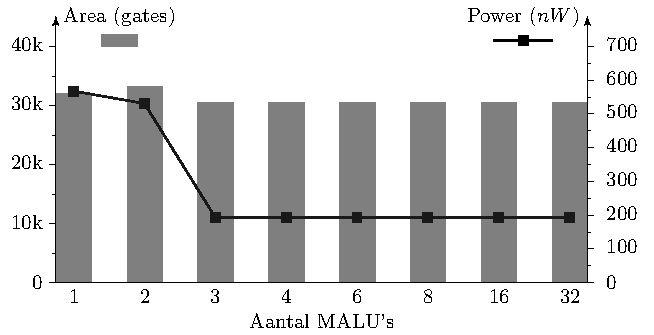
\includegraphics[scale=1]{results-md}}
		\caption{Syntheseresultaten voor implementaties met meerdere MALU's\label{figuur-resultaten-md}}
\end{figure}

\section{Hogere kloksnelheid vs.\ meerdere MALU's}

Aan de gegeven kloksnelheid van 10kHz doet een schakeling met \'e\'en MALU er 51.5 seconden over om \'e\'en pairing te berekenen. Dit zal  in de meeste gevallen onaanvaardbaar zijn. Daarom wordt hier onderzocht wat de effecten op de schakeling zijn indien de kloksnelheid wordt opgedreven en er eventueel meerdere MALU's gebruikt worden. Aangezien het doel nog steeds blijft de schakeling zo klein mogelijk te maken, zal voor een implementatie met meerdere MALU's enkel die met twee nader onderzocht worden.

Stel een maximale rekentijd $t_{\text{max}} = 50ms$. Voor een implementatie met \'e\'en MALU moet de klokfrequentie $f_1$ dan 1030 maal verhoogd worden. Wanneer men de schakeling met twee MALU's even snel wenst te maken als die met \'e\'en dan dient de kloksnelheid $f_2$ van die eerste vermenigvuldigd te worden met:
\[\begin{aligned}
\Delta f &= \frac{272484}{514917}\\
	&\approx 0.53.
\end{aligned}\]
De kloksnelheden van de respectievelijke schakelingen zijn dan:
\[\begin{aligned}
f_1	&= 10.3\text{MHz}\\
f_2	&\approx 5.45\text{MHz}.
\end{aligned}\]

Ter vergelijking worden de resulterende parameters van beide implementaties gegeven in \reftbl{tabel-resultaten-m1-vs-m2}. Beiden werden volledig gehersynthetiseerd met aangepaste parameters voor de klok. Vandaar dat de opgegeven grootte enigzins verschilt met eerder gegeven resultaten. De schattingen voor het vermogen zijn dus ook niet bekomen door de conversie formule aan het begin van dit hoofdstuk toe te passen. Welke van de twee opties de voorkeur zal genieten, zal afhangen van toepassing tot toepassing.

\begin{table}[h]
	\caption{Vergelijking van syntheseresultaten voor twee verschillende implementaties die er even lang over doen \'e\'en pairing te berekenen}
	\label{tabel-resultaten-m1-vs-m2}

	\centering
	\begin{tabular}{lll@{$\;\;$}l}
		\toprule
		& 1 MALU	& \multicolumn{2}{l}{2 MALU's}\\
		\midrule
		Opp. (gates)				& $30\,481$	& $30\,481$	& 120\% \\
		$f$ (MHz)					& 10.3		& 5.45		& 52.9\% \\ 
		Verbruik ($nW$)			& 				& 				& \\
		$\quad$ Dynamisch			& 104			& 134			& 118\% \\
		$\quad$ Leakage			& 114			& 164			& 144\% \\
		$f_{\text{max}}$ (MHz)	& 47.73		& 40.12		& 85\% \\
		\bottomrule	
	\end{tabular}
\end{table}

\section{Vergelijking met bestaande implementaties}

Gezien de vrij recente ontdekking van pairings lag de focus tot nu toe vooral op het snel berekenen van de pairing. Enkele papers beschrijven een ontwerp voor gebruik in sensor netwerken. Helaas hebben deze als doelplatform allemaal een microprocessor. Er werden slechts drie papers gevonden gevonden in de literatuur waarin het uiteindelijke resultaat naar een ASIC gesynthetiseerd werd. Alle andere  gepubliceerde implementaties werden ontwikkeld in software of voor FPGA's.

Het is dus zo goed als onmogelijk een grondige vergelijking te maken tussen de verschillende bestaande implementaties. Toch zal zo goed als mogelijk getracht worden enigszins een overzicht te geven, zodat de in deze thesis voorgestelde schakeling beter geplaats kan worden.

De ontwerpen specifiek gericht op sensor netwerken worden voorgesteld in \cite{tinypbc, tinytate, nanoecc}. In alle gevallen wordt de pairing berekend op een ATMega128L microchip. Deze implementaties zijn ontwikkeld voor gebruik op een MICA node, specifiek ontwikkeld voor gebruik in sensor netwerken. Een overzicht van de resultaten is gegeven in \reftbl{tabel-resultaten-sensor}. Rekening houdend met het stroomverbruik gegeven in \cite{nanoecc} wordt het verbruik geschat op ongeveer $23.60mW$. Uiteraard zijn de oppervlakte en het verbruik van een microchip implementatie niet te vergelijken met de in deze thesis voorgestelde ASIC schakeling, gezien de zeer verschillende architectuur en de filosifie achter het gebruik van beiden.

\begin{table}[h]
	\caption{Resultaten uit de literatuur voor ontwerpen met focus op sensor netwerken}
	\label{tabel-resultaten-sensor}

	\centering
	\begin{tabular}{lllll}
		\toprule
		&	\multicolumn{2}{c}{NanoECC \cite{nanoecc}}	& \multirow{2}{*}{TinyTate \cite{tinytate}}	& \multirow{2}{*}{TinyPBC \cite{tinypbc}}\\
		\cmidrule(r){2-3}
		& Binair	& Priem	&	& \\
 		\midrule
		Veld					& $\mathbb{F}_{2^{163}}$	& $\mathbb{F}_{p}$ 160 bit	& $\mathbb{F}_{p}$ 256 bit	& $\mathbb{F}_{2^{271}}$ \\
		Pairing				& Tate							& Tate							& Tate							& $\eta_T$ \\
		Rekentijd ($s$)	& 	10.96							& 17.93							& 30.21							& 5.45\\
		\bottomrule
	\end{tabular}
\end{table}

In de literatuur zijn vrij veel ontwerpen voor FPGA's terug te vinden. Het probleem is echter dat men zich bij het ontwerp hiervan steeds toelegt op het behalen van een zo hoog mogelijke snelheid, wat resulteert in een grote oppervlakte. Ook wordt vaak gerekend over grote velden (bv. $\mathbb{F}_{2^{313}}$ of $\mathbb{F}_{3^{197}}$), wat meer veiligheid biedt, maar resulteert in nog grotere ontwerpen.

Grootte van een FPGA ontwerp wordt vermeld in \emph{slices} (Xilinx) of \emph{logic elements} (Altera). Deze eenheden zijn onmogelijk om te zetten naar een aantal gates. Zodoende is het dus niet mogelijk de grootte van deze ontwerpen te vergelijken met die van een ASIC schakeling.

Toch wordt in \reftbl{tabel-resultaten-fpga} een sumier overzicht gegeven van een zeer beperkt aantal ontwerpen. Bij de selectie hiervan werd vooral gekozen voor ontwerpen waarin in een vrij klein veld gerekend werd. Er dient in acht te worden genomen dat bij al deze implementaties snelheid, en niet oppervlakte, het voornaamste doel is. Het gebruik van een vermenigvuldigingsschakeling equivalent aan het gebruik van honderd of meer MALU's is in deze gevallen eerder regel dan uitzondering.

\begin{table}[h]
	\caption{Resultaten uit de literatuur voor ontwerpen ontwikkeld voor FPGA's}
	\label{tabel-resultaten-fpga}

	\centering
	\begin{tabular}{llllll}
		\toprule
		&	\multicolumn{1}{c}{Veld}	& \multicolumn{1}{c}{Pairing}	& $\begin{array}{@{}c@{}}\text{Opp.}\\\text{[slices]}\end{array}$	& $\begin{array}{@{}c@{}}f\\\text{[MHz]}\end{array}$	& $\begin{array}{@{}c@{}}\text{Reken-}\\\text{tijd }[\mu s]\end{array}$\\
		\midrule
		Ronan \emph{et al.} \cite{ronan}				& $\mathbb{F}_{2^{103}}$	& Mod. Tate	& 21021	& 51	& 206\\
		Shu \emph{et al.} \cite{shu}					& $\mathbb{F}_{2^{239}}$	& Mod. Tate	& 25287	& 84	& 41\\
		Keller \emph{et al.} \cite{keller}			& $\mathbb{F}_{2^{251}}$	& Mod. Tate	& 27725	& 40	& 2370\\
		Grabher and Page \cite{grabher}				& $\mathbb{F}_{3^{97}}$		& Mod. Tate	& 4481	& 150	& 432\\
		Beuchat \emph{et al.} \cite{beuchat-eta}	& $\mathbb{F}_{3^{97}}$		& $\eta_T$	& 1833	& 145	& 192\\
		\bottomrule
	\end{tabular}
\end{table}

Ten slotte rest dan nog de vergelijking met de tot nu toe gepubliceerde ASIC ontwerpen uit \cite{beuchat-asic}, \cite{kammler} en \cite{savas}. Zowel in \cite{beuchat-asic} als \cite{savas} wordt met het oog op het behalen van zo hoog mogelijke snelheden ontworpen. De implementatie uit \cite{kammler} bevat naast de schakeling voor pairings tevens een RISC processor. \reftbl{tabel-resultaten-asic} geeft een vergelijkend overzicht van het ontwerp voorgesteld in deze thesis en de ontwerpen uit \cite{beuchat-asic} en \cite{kammler}.

\begin{table}[h]
	\caption{Vergelijking van het ontwerp voorgesteld in deze thesis met ASIC ontwerpen uit de literatuur}
	\label{tabel-resultaten-asic}

	\begin{narrow}{-1cm}{-1cm}
		\centering
		\begin{tabular}{llllll}
			\toprule
			&	\multicolumn{2}{c}{Thesis (1 MALU, CG 3)}	& \multirow{2}{*}{PairingLite \cite{beuchat-asic}}	& \multicolumn{1}{c}{\multirow{2}{*}{$\begin{array}{@{}c@{}}\text{Kammler}\\\text{\emph{et al.} \cite{kammler}}\end{array}$}}	&  \multicolumn{1}{c}{\multirow{2}{*}{$\begin{array}{@{}c@{}}\text{K\"om\"urc\"u en}\\\text{Savas \cite{savas}}\end{array}$}}\\
			\cmidrule(r){2-3}
			& \multicolumn{1}{c}{10kHz} & \multicolumn{1}{c}{10.3Mhz} & & &\\
	 		\midrule
			Veld							& $\mathbb{F}_{2^{163}}$	& $\mathbb{F}_{2^{163}}$	& $\mathbb{F}_{3^{97}}$	& $\mathbb{F}_{p}$ 256 bit	& $\mathbb{F}_{3^{97}}$ \\
			Pairing						& Tate							& Tate							& $\eta_T$					& Optimal Ate 					& Tate\\
			Technologie					& $0.13 \mu m$					& $0.13 \mu m$					& $0.18 \mu m$				& $0.13 \mu m$					& $0.25 \mu m$\\
			Opp. [gates]				& $27\,734$						& $27\,734$						& $193\,765$				& $97\,000$						& \emph{$10mm^2$}\footnotemark[2]\\
			$f$ [MHz]					& 0.01							& 10.3							& 200							& 338								& 78\\
			Rekentijd [$\mu s$]		& $51.5 \cdot 10^6$			& $50 \cdot 10^3$				& 46.7						& 15800							& 250\\
			Verbruik [$mW$]			& $206 \cdot 10^{-6}$		& $212 \cdot 10^{-3}$		& 672							& ?								& ?\\
			Opp. $\cdot$ tijd\footnotemark[3]			& \\
			Opp. $\cdot$ verbruik	& \\
			\bottomrule		
		\end{tabular}
	\end{narrow}
		
	\raggedright \footnotesize \footnotemark[2] Voor deze implementatie zijn geen gegevens voorradig i.v.m.\ het aantal gates. De gegeven oppervlakte is die van de complete schakeling inclusief routing.
	
	\footnotemark[3] Bij de berekening van deze waarde werd het bekomen getal gedeeld door de kloksnelheid. Hoewel de oppervlakte enigszins afhangt van de klokfrequentie, za
\end{table}
